

\numbertable{
    \begin{tabular}{lrr}
    Sector & \multicolumn{1}{l}{Name} & Polygon Length \\  \midrule
    \multirow{6}[0]{*}{\passage{Tolminska Korita}} & \multicolumn{1}{l}{\passage{Black Knight}} & 116.08 m \\
        & \multicolumn{1}{l}{\passage{Korita}} & 86.39 m \\
        & \multicolumn{1}{l}{\passage{Crack in Time}} & 44.60 m \\
        & \multicolumn{1}{l}{\passage{Sidewinder}} & 23.86 m \\
        & \multicolumn{1}{l}{\passage{Stalemate}} & 35.73 m \\
        & \multicolumn{1}{l}{\passage{White Bishop}} & 52.86 m \\ \midrule
    \multirow{6}[0]{*}{Southwards of \passage{Cheetah}} & \multicolumn{1}{l}{\passage{Kamikaze}} & 159.60 m \\ 
        & \multicolumn{1}{l}{\passage{Lost Hopes}} & 35.62 m \\
        & \multicolumn{1}{l}{\passage{Mudstone}} & 53.36 m \\
        & \multicolumn{1}{l}{\passage{Rolling Stones}} & 48.27 m \\
        & \multicolumn{1}{l}{\passage{Surprise}} & 71.24 m \\
        & \multicolumn{1}{l}{\passage{Wonderland}} & 134.29 m \\ \midrule
    \multirow{4}[0]{*}{Northwards of \passage{Cheetah}} & \multicolumn{1}{l}{\passage{Consort}} & 239.99 m \\
        & \multicolumn{1}{l}{\passage{Esoterica}} & 63.24 m \\
        & \multicolumn{1}{l}{\passage{It Will Rain}} & 48.92 m \\
        & \multicolumn{1}{l}{\passage{Serpentine}} & 70.53 m \\ \midrule
    \multirow{3}[0]{*}{\passage{Palace of King Minos} (climb from the \passage{Albert Hall})} & \multicolumn{1}{l}{\passage{Palace}} & 589.63 m \\
         & \multicolumn{1}{l}{\passage{Povodni Mož}} & 27.69 m \\
         & \multicolumn{1}{l}{\passage{Povodni Mož 2}} & 161.20 m \\ \midrule    
    Below \passage{Republica} & \multicolumn{1}{l}{\passage{Insomnia}} & 100.30 m \\ \midrule         
         &       &  \\        
\textbf{Total} & & \textbf{2163.40 m} \\         
\end{tabular}
}



\subsection{Vrtnarija Loop Closures}

Our survey is now corrected to grid north based on the NOAA American
Webservice, with Lat + Long on \passage{M10}/\passage{Bivi}, calculated for 1st Aug of each year.
This was mainly to agree with surface DEM data \& GPS data (declination is
approximately 2.5 degrees), as the rate of change of declination is slow (6
minutes a year).

\passage{Vrtnarija} now possesses two large loops, making the cave into a `figure 8' configuration. 

During 2009 the \passage{Captain Kangaroo} --- main pitch series loop was closed
(consisting of data collected from 2000--2009, approximately 1.8km loop).
During 2010 the \passage{Tolminska Korita} -- \passage{Big Rock} loop was closed (data from
2001--2010, approximately 1.7km loop).

All sampled misclosures were 1.5--2.0 \%. Typically the horizontal misclosure
was twice that of the vertical (our total plan length of survey polygon is also
approximately double the total vertical length).




\begin{pagesurvey}
\centering
\frame{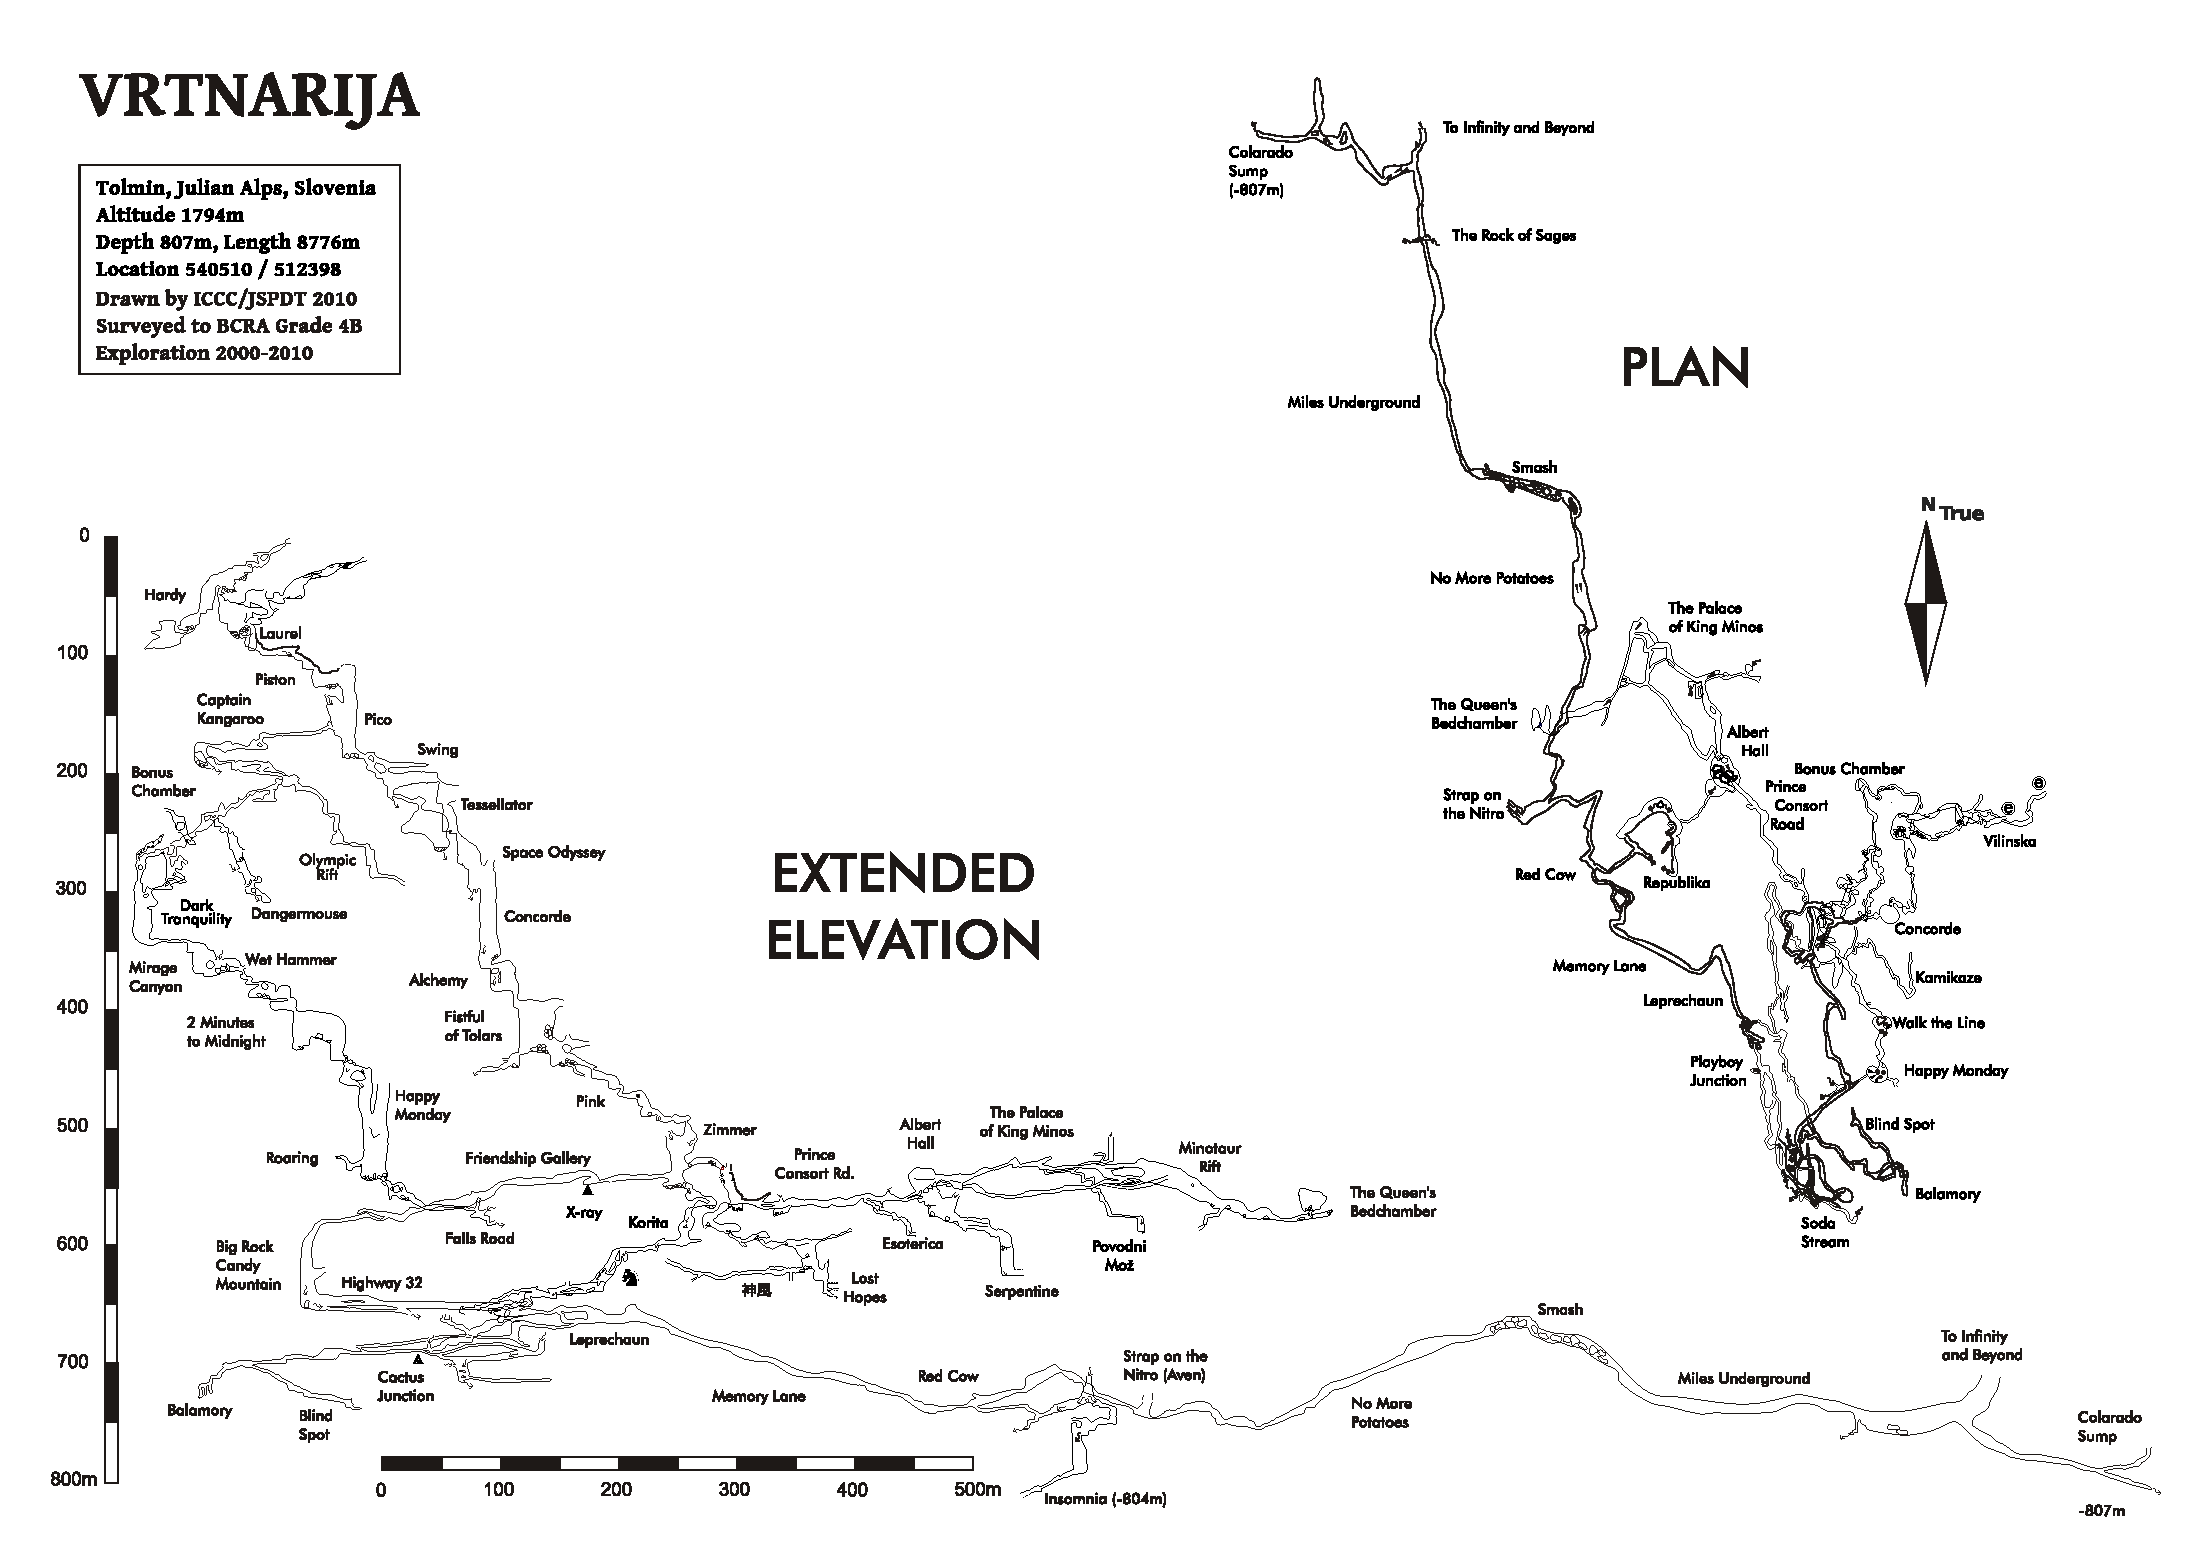
\includegraphics[width=\textheight, angle=90]{2010/survey/gw_2011-01-31.pdf}}
\caption[2010 Vrtnarija Survey]{2010 \passage{Vrtnarija} Survey}
\end{pagesurvey}


\begin{pagesurvey}
\centering
\frame{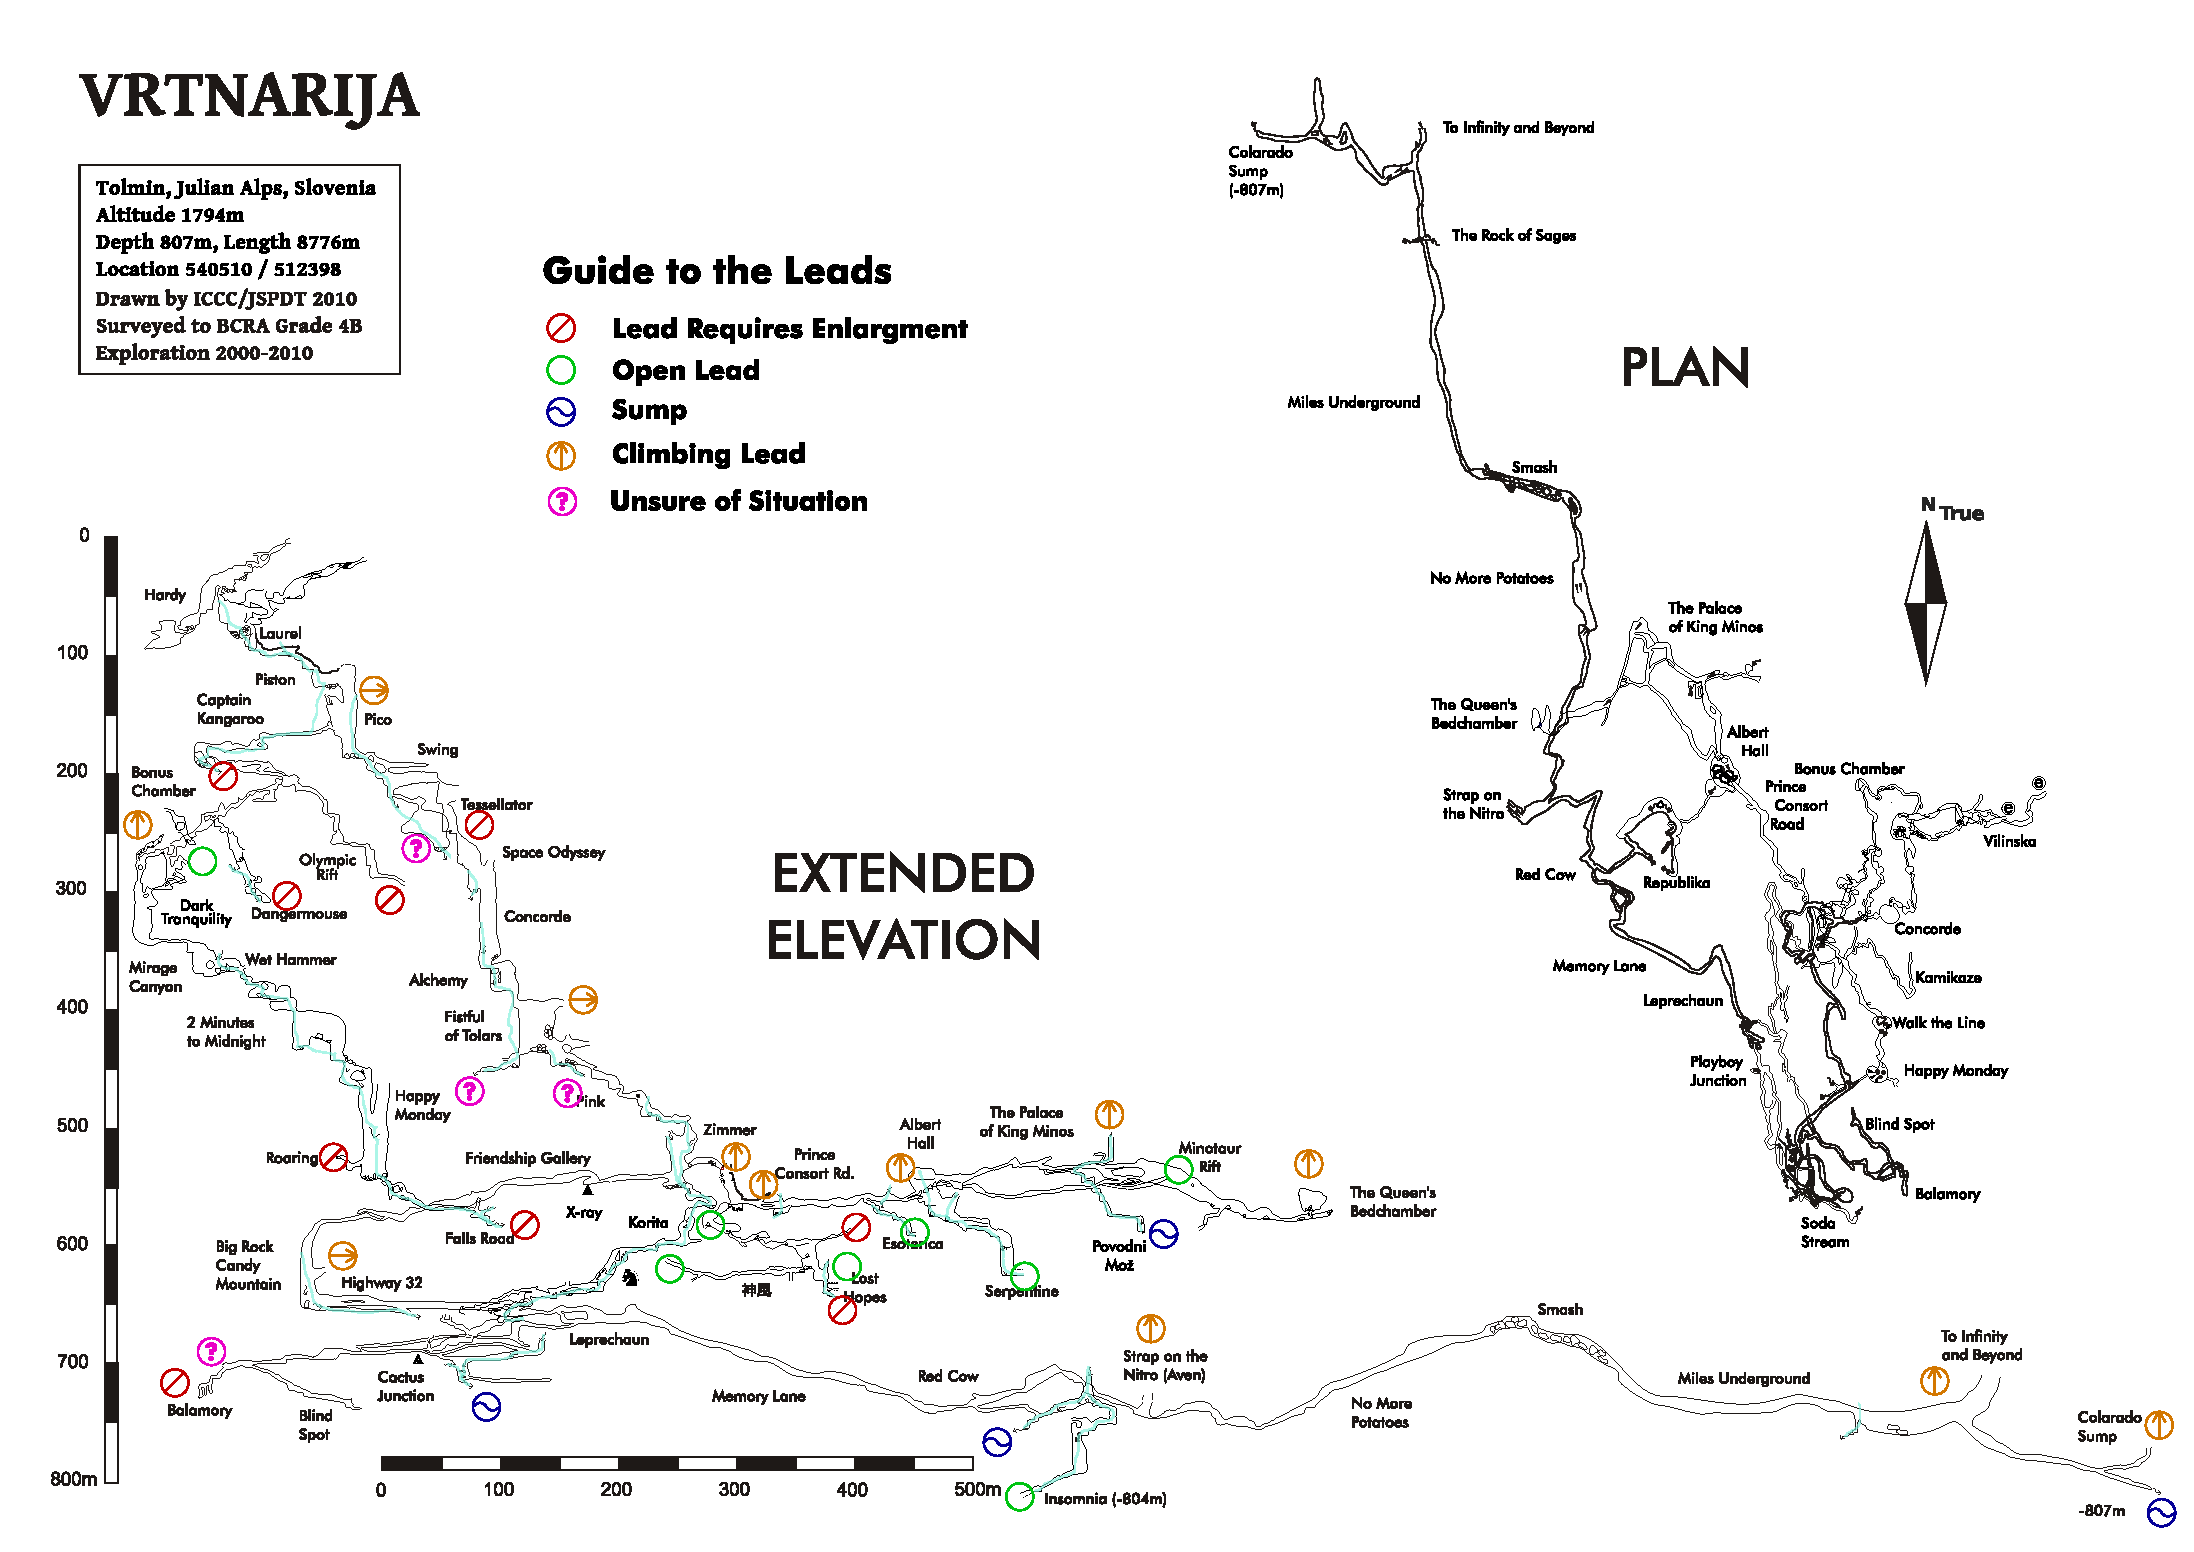
\includegraphics[width=\textheight, angle=90]{2010/survey/gw_2011-01-31-leads_water.pdf}}
\caption[2010 Vrtnarija Survey with Leads and Water Highlighted]{2010 \passage{Vrtnarija} Survey  with Leads and Water Highlighted}
\end{pagesurvey}